% Thesis-ready LaTeX condensation of RT_NCRNA_EMBEDDING_REPORT.md.
% The Markdown report is authoritative; this carries the same frozen numbers in a form that
% drops into a thesis chapter. Compile: pdflatex RT_NCRNA_EMBEDDING_REPORT.tex
\documentclass[11pt,a4paper]{article}
\usepackage[margin=2.5cm]{geometry}
\usepackage{booktabs,graphicx,microtype,longtable}
\usepackage[hidelinks]{hyperref}
\usepackage[table]{xcolor}
\title{Cross-modal information in frozen RT and ncRNA sequence representations}
\author{Melissa Rios \\ \small retron reverse transcriptase $\leftrightarrow$ retron ncRNA, embedding track}
\date{2026-09-18}
\begin{document}\maketitle

\begin{abstract}
We asked whether naturally associated retron reverse transcriptase (RT) and ncRNA sequences
carry cross-modal information distinguishing their observed association beyond composition,
sequence relatedness, retron type and dataset structure. Using frozen ESM-C 300M and RiNALMo
giga-v1 representations over 30{,}924 observed associations, a regularized CCA probe retrieves
the observed partner far above chance against random candidates (MRR $0.4407$ vs $0.0900$;
permutation $p=0.0005$) and above length/GC-matched candidates. When candidate ncRNAs are
restricted to the query's retron type, the improvement over a k-mer baseline is no longer
statistically distinguishable ($+0.0298$, 95\,\% CI $[-0.0048,+0.0633]$). Cross-modal
neighbourhoods are type-associated rather than pair-specific: the observed partner is the nearest
neighbour for $0.56\,\%$ of queries (median rank 238 of 2{,}756), while $50\,\%$ of top-10
neighbours share the query's retron type against $9.4\,\%$ prevalence. We conclude that
system/type-level organization has evidence while individual partner specificity does not, and
that the binding constraint is independent relatedness components ($n_{\mathrm{eff}}=14.1$), not
model capacity.
\end{abstract}

\section{Question and claim boundary}
\emph{Do naturally associated retron RT and ncRNA sequences contain cross-modal sequence
information that distinguishes their observed association beyond trivial sequence composition,
relatedness, retron type and dataset structure?} This is not a test of co-evolution, physical
binding, biochemical compatibility, or residue--nucleotide contacts. Combinations recorded
together are \emph{observed / natural associations}, not experimentally validated positives;
combinations absent from the corpus are \emph{non-observed pairings}, not incompatible ones.

\section{Population}
30{,}924 observed pairs over 29{,}192 unique RT and 16{,}458 unique oriented ncRNA sequences,
21 retron types (\texttt{rt\_ncrna\_exact\_pairs\_v1}, Stage-1 gate \texttt{dbchar\_g3}). Tiers:
T1 30{,}287; T2 25{,}673; T3 23{,}680; T4 7{,}476. ncRNA sequences were reconstructed for this
track and verified \textbf{16{,}458/16{,}458} by SHA-256 round-trip against the Stage-1 hash,
which is itself the hash of the \emph{oriented} sequence. RT 21--2{,}860\,aa (median 370);
ncRNA 34--395\,nt (median 151). One ncRNA is observed with 705 distinct RTs, which is why
false-candidate exclusion is mandatory.

\section{Representations}
Frozen pretrained encoders, no weights updated: ESM-C 300M ($960$-d pooled, 29{,}192 sequences)
and RiNALMo giga-v1 ($1280$-d pooled, 16{,}458 sequences), produced on Ibex A100 with per-shard
provenance and no truncation. Token-level arrays (21\,GB and 6.6\,GB) are retained but
\emph{unused} pending independently established msr/msd and RT-domain annotations. Pooled frozen
embeddings were chosen as the lowest-capacity first probe because the effective sample size is
small, the probe is interpretable, and it sets the floor that any escalation must clear.

\section{Relatedness-aware split}
RT clusters: \texttt{mmseqs easy-cluster --min-seq-id 0.50 -c 0.8 --cov-mode 0} (bidirectional
80\,\% coverage). ncRNA clusters: \texttt{cd-hit-est -c 0.80 -aS 0.8 -n 8 -T 1} (shorter-sequence
80\,\% coverage). The split unit is a \textbf{connected component of the bipartite RT-cluster
$\leftrightarrow$ ncRNA-cluster graph}, indivisible; allocation is deterministic with no RNG.

\begin{table}[h]\centering\small
\begin{tabular}{lrrrrr}\toprule
fold & pairs & \% & components & $n_{\mathrm{eff}}$ & T4 (\%) \\\midrule
train & 21{,}647 & 70.00 & 361 & 6.4 & 72.34 \\
validation & 4{,}639 & 15.00 & 357 & 14.2 & 14.41 \\
\textbf{test} & \textbf{4{,}638} & 15.00 & 357 & \textbf{14.1} & 13.26 \\\bottomrule
\end{tabular}\caption{The frozen split. $n_{\mathrm{eff}}=(\sum_i s_i)^2/\sum_i s_i^2$ is the
effective number of independent components and is the inference unit; 4{,}638 pairs are
\emph{not} 4{,}638 observations.}\end{table}

Threshold selection was performed blind to any compatibility result. Strict blocking and
statistical power are in direct opposition in this universe: RT $0.30$ blocks leakage to
$1.7\,\%$ but leaves a single-component validation fold, while RT $\geq 0.70$ gives hundreds of
effective units at $\sim 90\,\%$ leakage. Leakage was measured with an \emph{independent}
instrument (mmseqs $-s\,7.5$; blastn word size 7) against a training-only database so censoring
is impossible. A near-duplicate sensitivity stratum (identity $\geq 0.90$, aligned coverage
$\geq 0.30$ with coverage symmetrized as $\max(q_{\mathrm{cov}},t_{\mathrm{cov}})$) was frozen;
structural ``fragment bridge'' remedies were priced and rejected because the best variant cost
$82\,\%$ of validation independence.

\begin{quote}\itshape The experiment evaluates generalization across the declared
sequence-relatedness component split. It does not establish generalization to evolutionarily
unrelated RT or ncRNA sequences.\end{quote}

\section{Task, models and baselines}
50-way retrieval (1 observed partner $+$ 49 retrieval decoys), chance MRR $0.0900$; any decoy
that is an observed partner of the query RT anywhere in the corpus is excluded and redrawn.
Baselines run first: \texttt{B-pop} (ncRNA-only marginal), \texttt{B-len}, \texttt{B-gc},
\texttt{B-kmer} (strongest trivial), \texttt{B-model} (RT-only marginal / retron-type label
shortcut). Cross-modal probe \texttt{M-CCA}: regularized CCA fit on training components only,
configuration $k=32,\ \alpha=0.01$ selected on validation rung-1 MRR over a predeclared 9-point
grid; test opened once.

\section{Results}
\begin{table}[h]\centering\small
\begin{tabular}{llrrlr}\toprule
rung & decoys matched on & \texttt{B-kmer} & \textbf{\texttt{M-CCA}} & 95\,\% CI & comps \\\midrule
1 & random & 0.2265 & \textbf{0.4407} & $[0.4039,0.4772]$ & 357 \\
2 & length + GC & 0.1418 & \textbf{0.2262} & $[0.1972,0.2565]$ & 316 \\
3 & \textbf{retron type} & 0.1534 & 0.1832 & $[0.1550,0.2126]$ & 299 \\
4 & ncRNA cluster & 0.0764 & 0.0925 & \textsc{undetermined} & 1 \\
5 & RT cluster & 0.1050 & 0.0992 & \textsc{undetermined} & 10 \\
6 & species & 0.1111 & 0.2982 & \textsc{undetermined} & 22 \\\bottomrule
\end{tabular}\caption{Retrieval across the candidate ladder. Intervals are component-level
bootstraps. Rungs 4--6 are \textsc{undetermined} --- absence of sufficient measurement, not
measured absence.}\end{table}

Paired per-component difference \texttt{M-CCA} $-$ \texttt{B-kmer}: rung 1 $+0.2142$
$[+0.1737,+0.2537]$; rung 2 $+0.0844$ $[+0.0503,+0.1187]$; \textbf{rung 3 $+0.0298$
$[-0.0048,+0.0633]$, not distinguishable}. Reverse direction (ncRNA$\to$RT) $0.4738$
$[0.4380,0.5104]$. Permutation failure control: observed $0.4407$ vs null mean $0.0901$,
$p=0.0005$. Near-duplicate-excluded population: $0.4329$ $[0.3910,0.4751]$, a $-0.008$ change.
Absence of a significant difference at rung 3 is \emph{not} proof of equivalence.

\section{Why: type-associated organization}
Observed-pair mean CCA cosine $0.3771$, against type-matched $0.3217$ (Cohen's $d=0.248$),
length/GC-matched $0.2803$ ($d=0.420$) and random $0.0872$ ($d=1.364$). In an open
2{,}756-candidate pool the observed partner is the nearest cross-modal neighbour for
$0.56\,\%$ of queries at median rank 238, while $51.9\,\%$ of nearest and $50.0\,\%$ of top-10
neighbours share the query's retron type against $9.4\,\%$ prevalence ($5.3\times$ enrichment).
The leading canonical dimension has correlation $0.9865$ with $\eta^2$ of retron type $0.809$
(RT) and $0.724$ (ncRNA). Retron type is recoverable from \emph{each modality alone} (ESM-C
$0.498$, RiNALMo $0.656$; majority $0.269$), supplying a sufficient route by which any
cross-modal alignment could score well without learning partner compatibility.

\begin{figure}[h]\centering
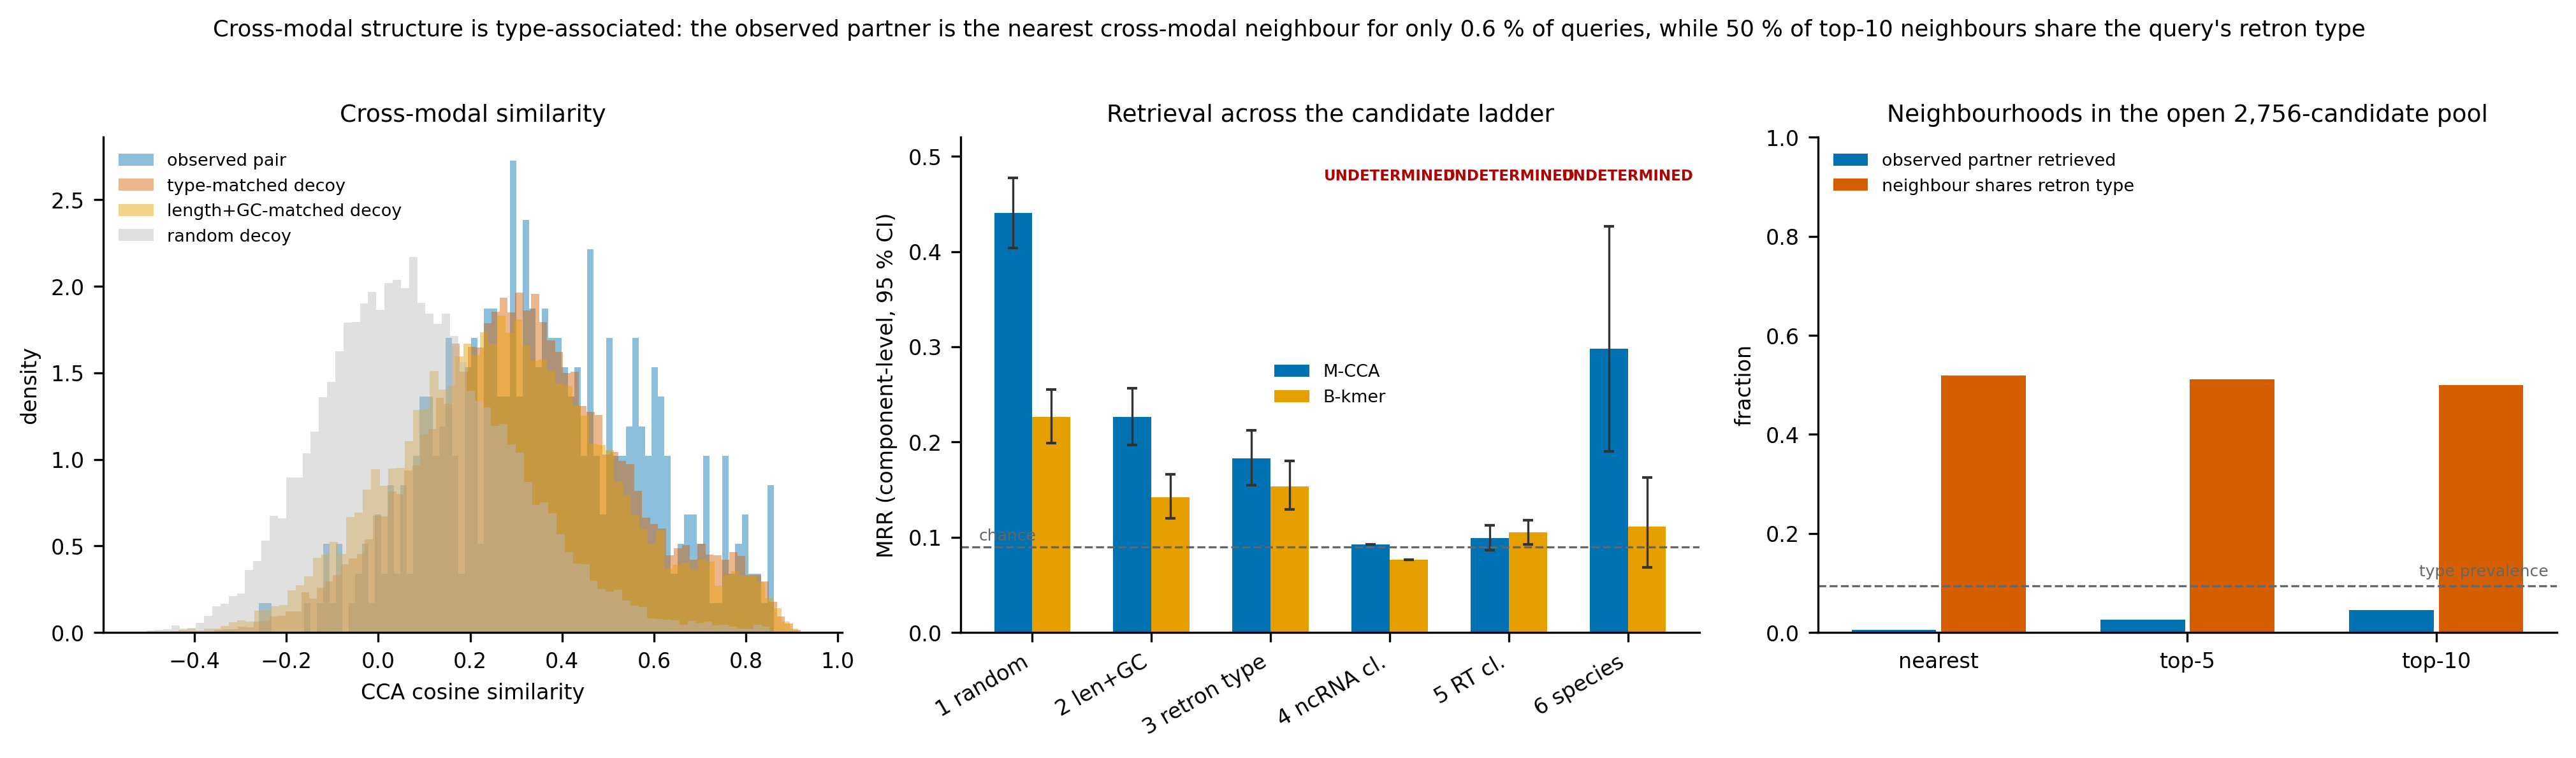
\includegraphics[width=\textwidth]{figures/fig4_similarity_retrieval.png}
\caption{(a) Cross-modal similarity for observed pairs and three decoy classes (descriptive).
(b) Retrieval across the candidate ladder with component-level intervals and rungs 4--6 marked
\textsc{undetermined} (inferential). (c) Neighbourhood composition in the open candidate pool
(descriptive).}\end{figure}

\begin{figure}[h]\centering
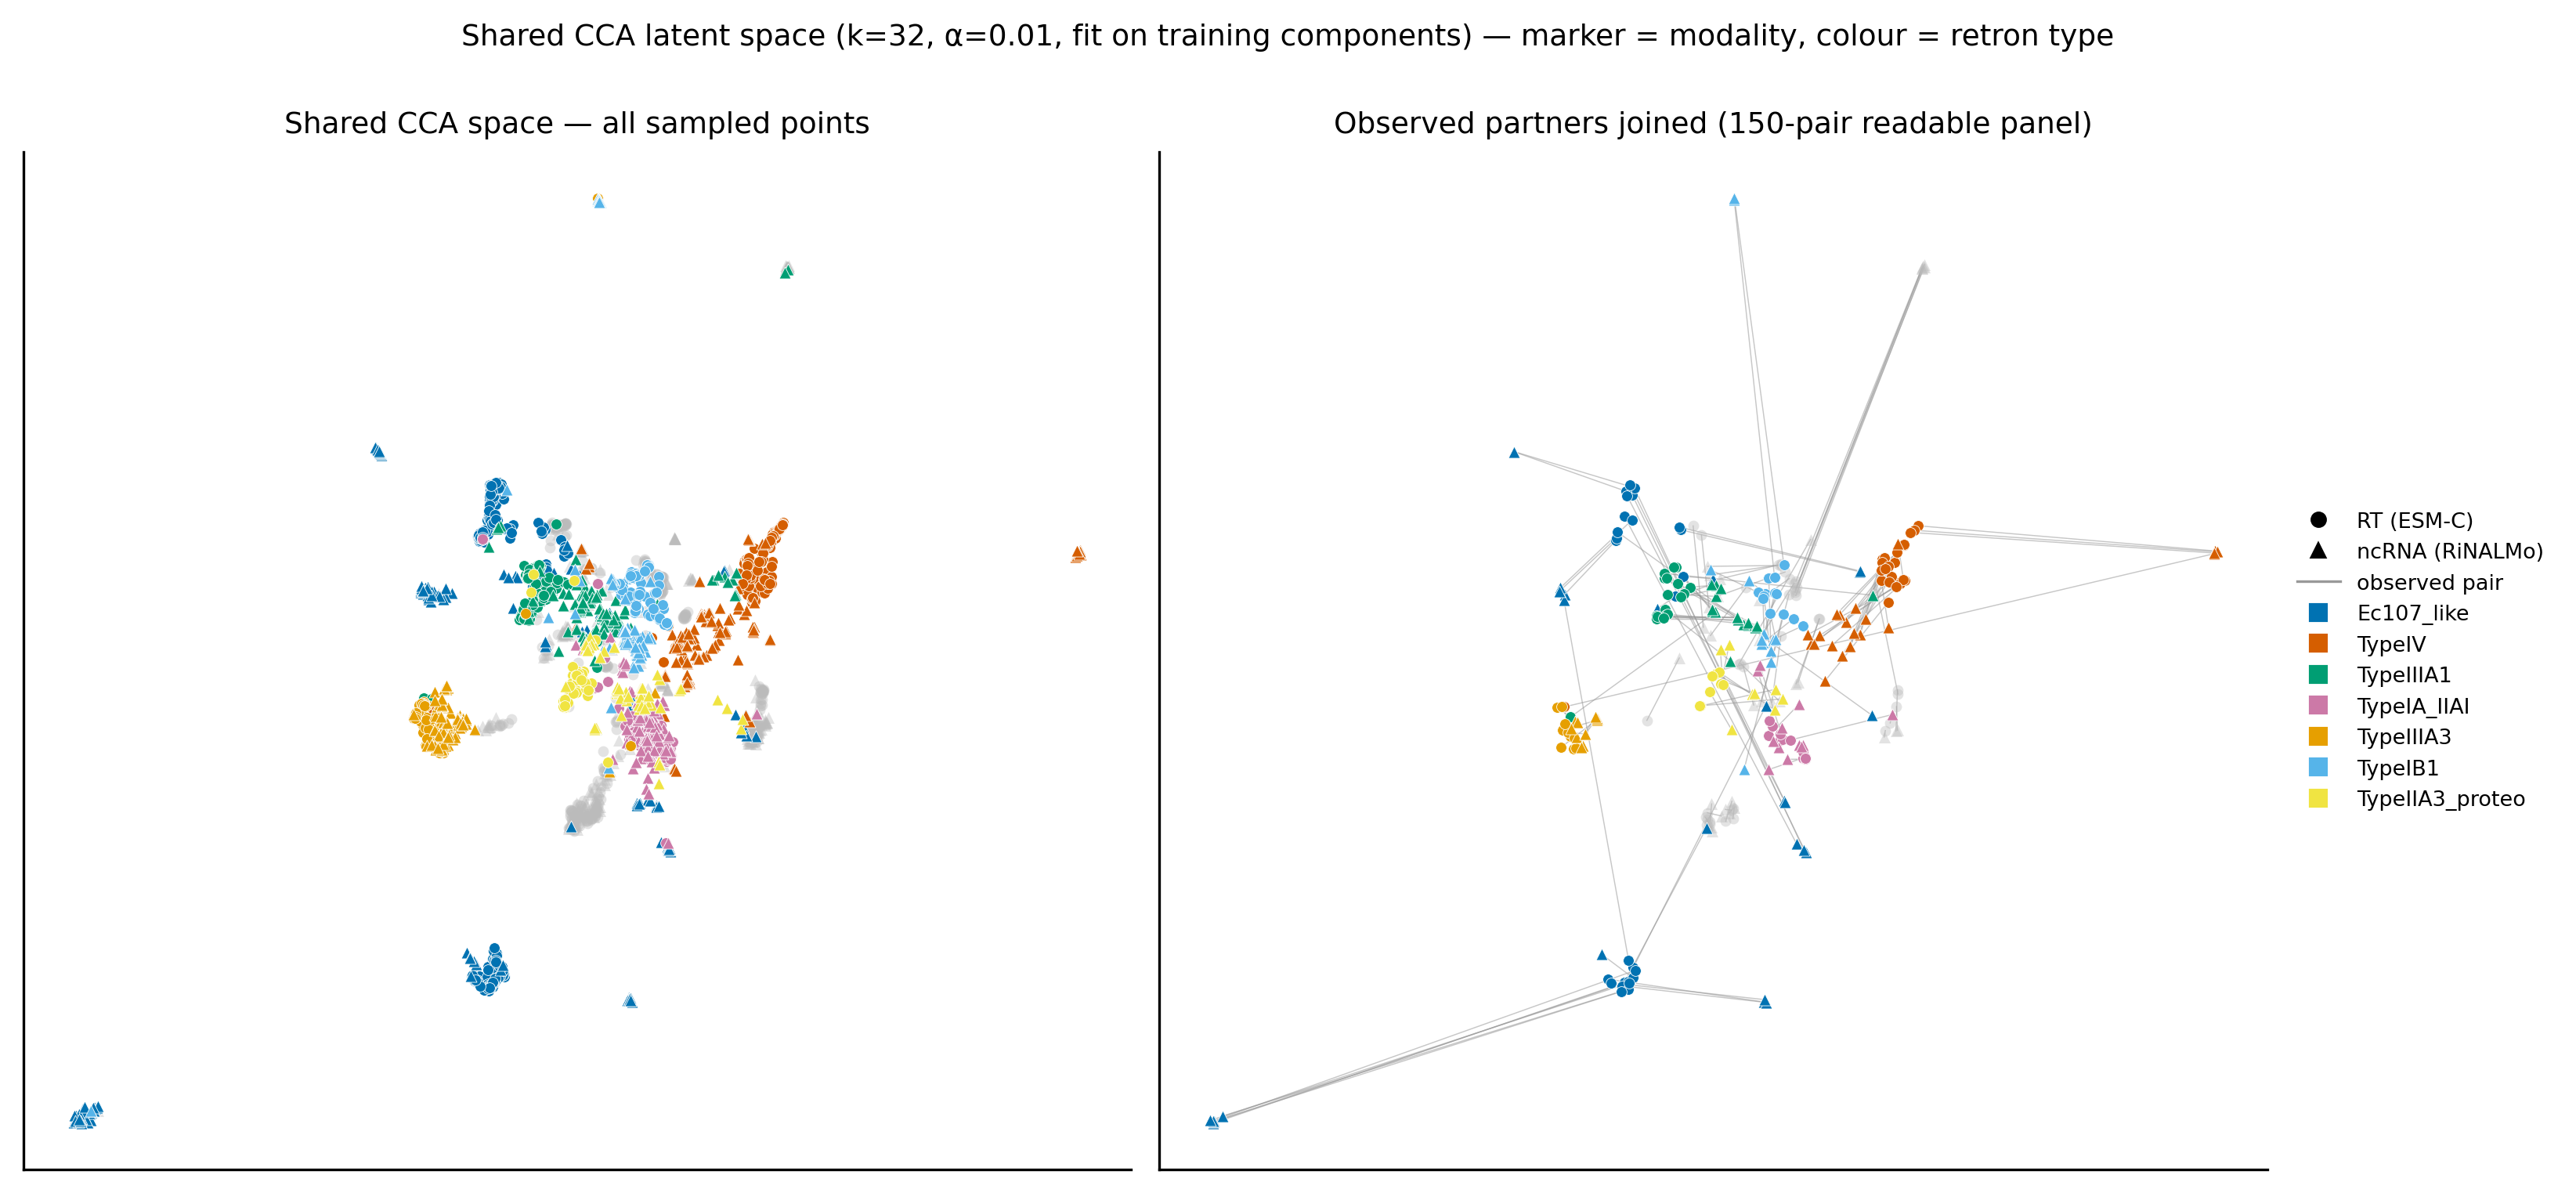
\includegraphics[width=\textwidth]{figures/fig3_shared_cca_atlas.png}
\caption{Shared CCA latent space; circles RT (ESM-C), triangles ncRNA (RiNALMo), colour retron
type, light segments joining observed partners in a readable 150-pair panel. UMAP layout is
visualization only and is not evidence of discrete biological classes.}\end{figure}

\section{Interpretation}
\begin{quote}\itshape Frozen ESM-C and RiNALMo representations contain substantial shared
structure associated with naturally occurring RT--ncRNA systems. This supports strong retrieval
against random and length/GC-controlled candidate sets. However, the present experiment does not
establish individual partner-specific compatibility beyond retron-type-associated structure: when
candidate ncRNAs are restricted by retron type, the M-CCA improvement over the k-mer baseline is
no longer statistically distinguishable.\end{quote}

This does \emph{not} prove that retron type explains all observed signal. Level 1 (shared
organization at retron-type / system-class level) has evidence; level 2 (individual partner
specificity) is not established.

\section{Why escalation stopped, and what would reopen it}
No InfoNCE, symmetric cosine contrastive, dual-encoder or cross-attention model was trained. The
pre-registered escalation condition was not met at rung 3, and with $n_{\mathrm{eff}}=14.1$ a
high-capacity model rewarded for type recognition could not be distinguished afterwards from one
that learned compatibility. Status: \textbf{not yet justified as a confirmatory partner-specific
test}, not \emph{method rejected}. An independent generative line of work in the same lab reached
the convergent conclusion that its model performs family rather than partner recognition, with a
contrastive arm that raised its optimised metric 43-fold while degrading the rank statistic.

A within-type design would remove type structure by construction. Of 21 retron types only
\texttt{TypeIIIA3} and \texttt{TypeIB1} meet the population criteria, and their \emph{test-fold}
$n_{\mathrm{eff}}$ are $3.7$ and $4.6$; \texttt{TypeIC1\_IC2} has 6{,}277 pairs but
$n_{\mathrm{eff}}=1.2$. The binding constraint is therefore independent relatedness components,
not model capacity or raw pair count --- a data and population-design problem. Because every
ncRNA call in the corpus derives from a covariance model, recovery of ncRNAs missed by CM-based
approaches would disproportionately add divergent, independent associations and should trigger
re-running the feasibility audit.

\end{document}
